\chapter{Webbdatabas för hantering av filer}
I detta kapitel kommer de olika delar som utvecklingen av systemet bestod av att presenteras. 

\section{Inledande möten}
Projektet inleddes med ett antal interna gruppmöten där projektets vision diskuterades utifrån projektets beskrivning. Diskussionen ledde till många frågor, dels kring tekniska bitar och dels kring kundens krav. På första kundmötet besvarades dessa frågor i den mån kunden kunde. Kunden hade inte alltid en bestämd åsikt om hur ett problem skulle lösas och lät därför utvecklarna hitta en lösning. Efter kundmötet hölls ett nytt gruppmöte där projektvisionen förtydligades och tekniska lösningar diskuterades och ritades upp. 

I inledningen av projektet diskuterades det mycket om hur systemet skulle utvecklas. Faktorer som språk och ramverk togs upp. Beslutet som fattades var att språket Ruby och ramverket Ruby on Rails skulle användas som grundstomme i projektet. Vidare användes också Javascript och ramverket Angularjs för att göra upplevelsen av systemet snabbare för användaren.

När gruppen hade en tydlig idé om hur databasen skulle se ut och vilken teknik som skulle användas skrevs en projektplan (se bilaga []) som skulle ligga till grund för arbetsrutinerna, ansvarsfördelningen och tidsplanneringen (se bilaga []).

\section{Hantering och strukturering av databaser}
Systemet använder sig utav en SQL-databas, där SQL står för \textit{Structured Query Language}. Det är ett programmeringsspråk för att lagra, bearbeta och hämta information i en databas \cite{sqlenc}.

\subsection{Databasstruktur}
Inledningvis togs en grundläggande databastruktur fram. Databasen innehöll användare, användares olika externa konton (till exempel Dropbox eller Google Drive), filer och taggar, se figur \ref{fig:relations}. 

\begin{figure}[!H]
\centering
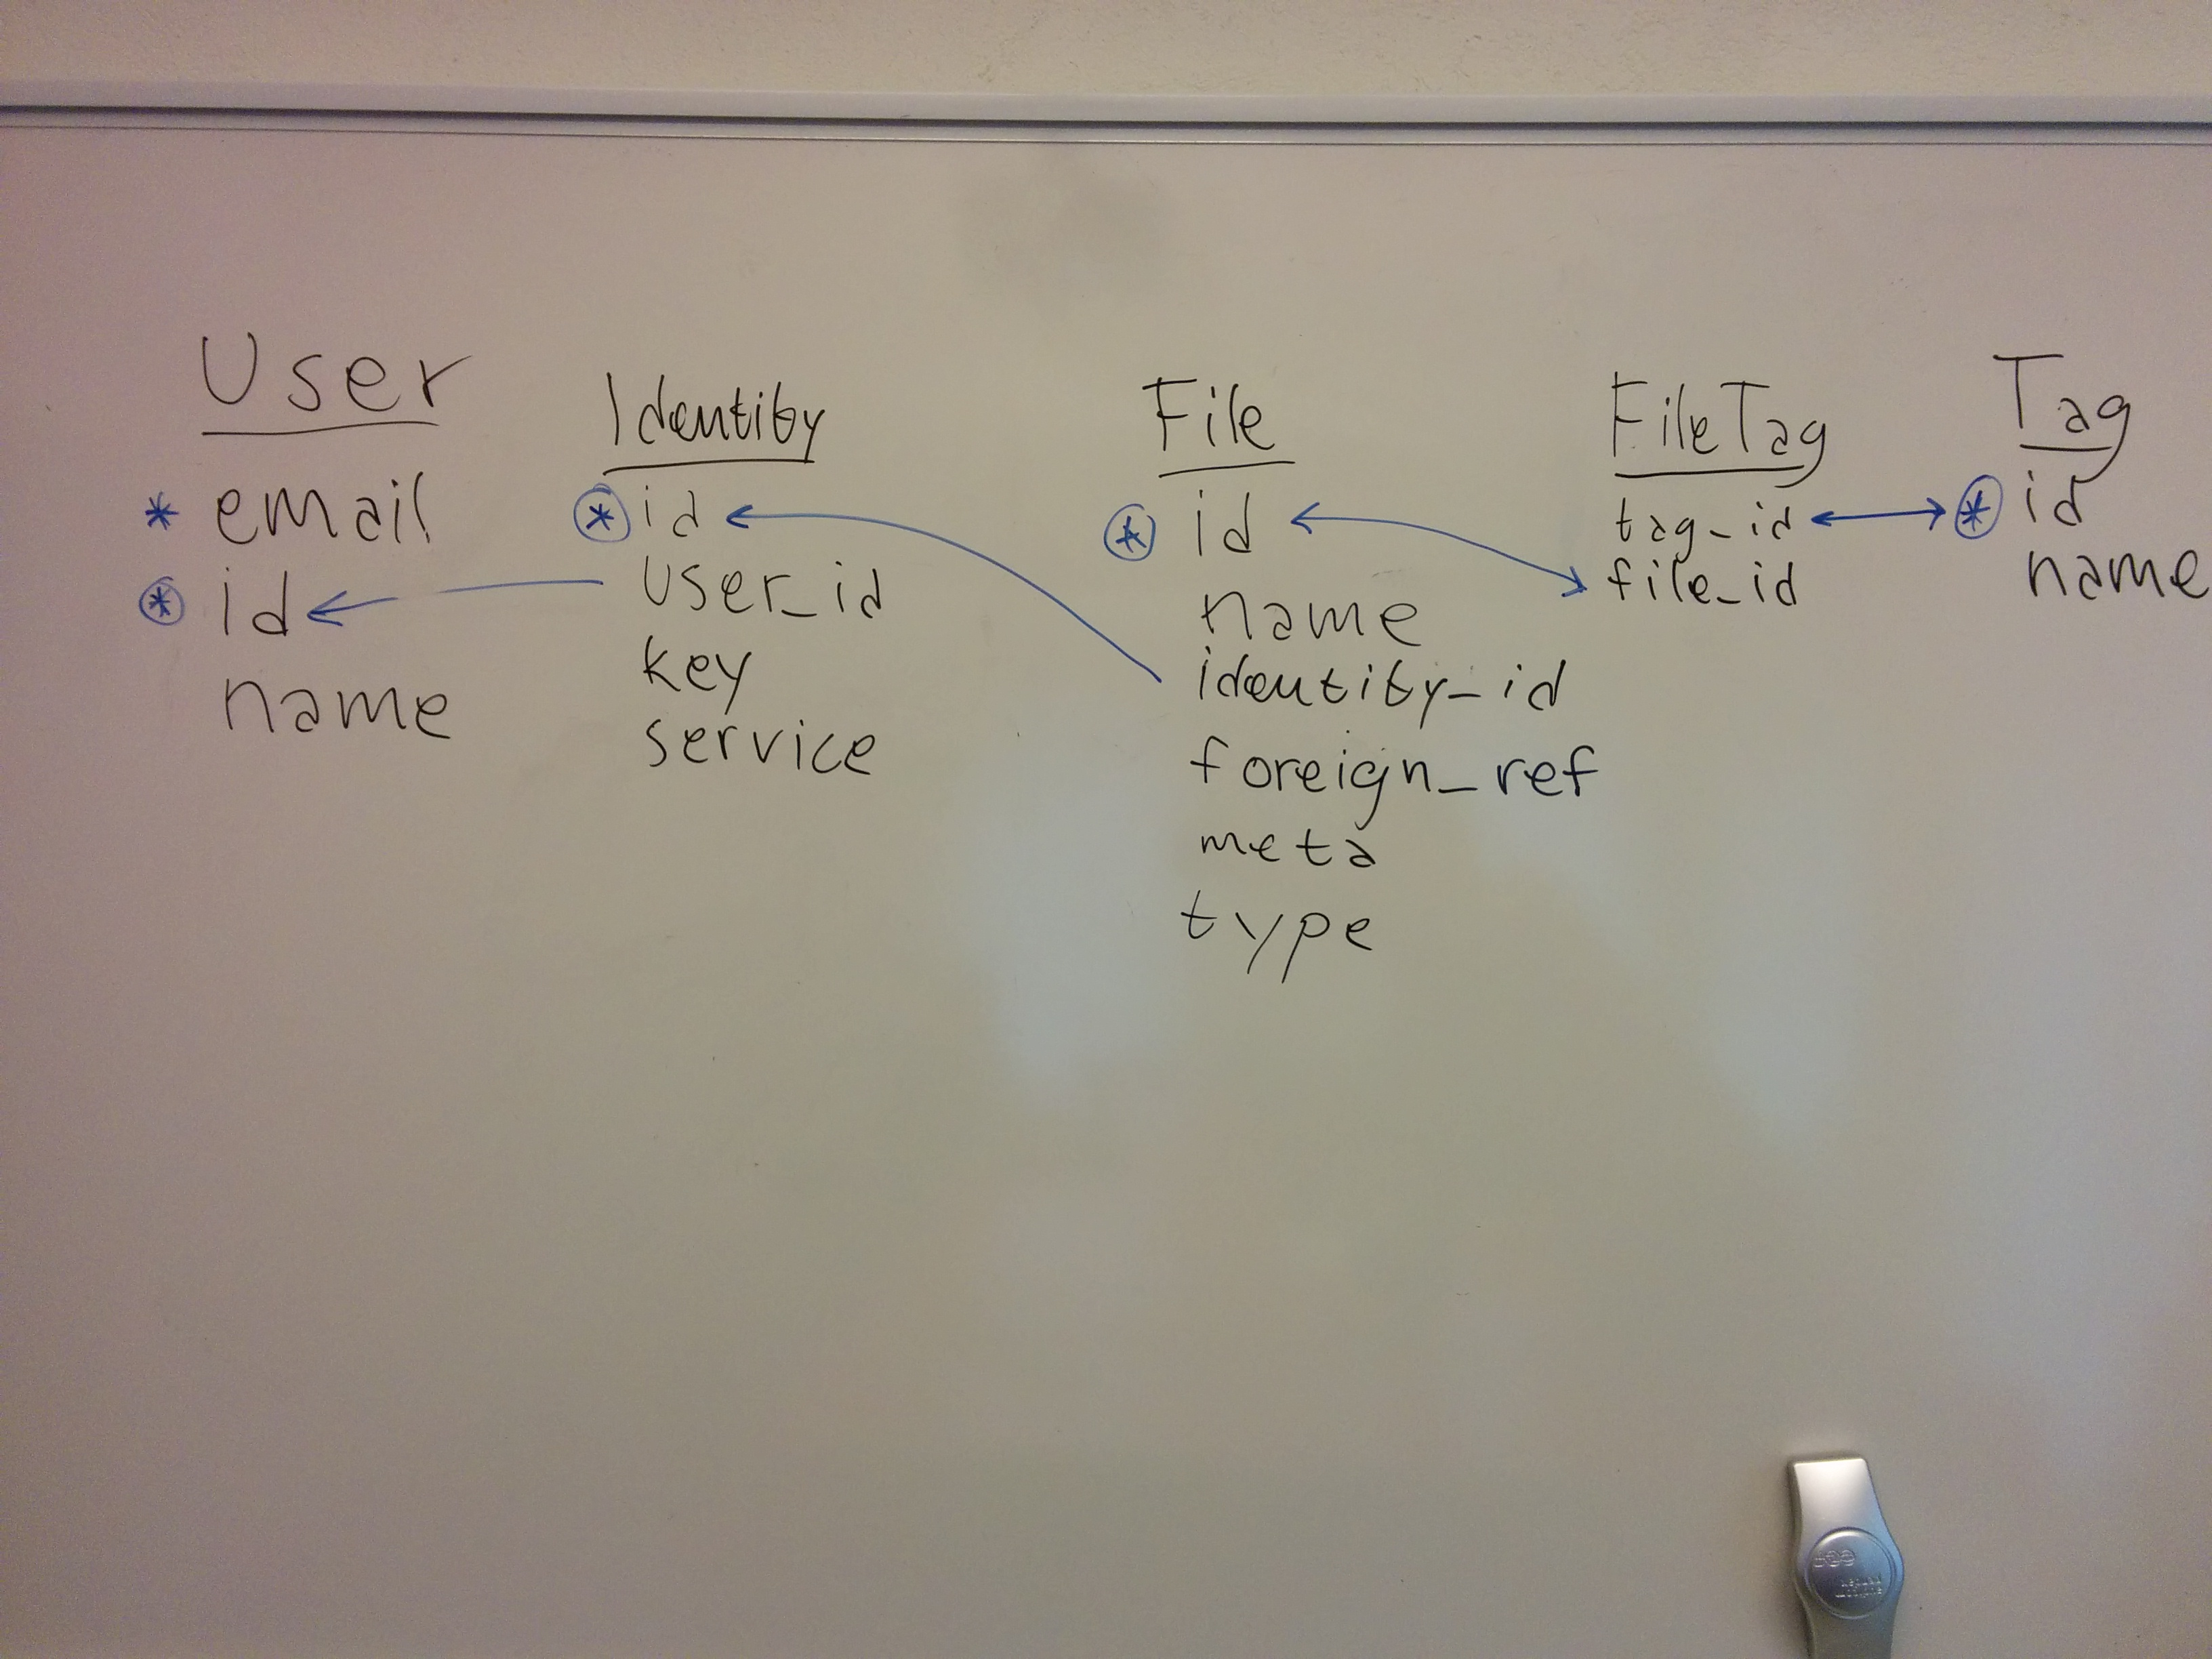
\includegraphics[width=0.8\textwidth]{figures/relations.jpg}
\caption{Visar strukturen för parametrarna \textit{parent} och \textit{child} i Google drive.}
\label{fig:relations}
\end{figure}

\subsection{Databashantering}
En stor komponent utav Ruby on Rails är modulen som heter \texttt{ActiveRecord}. Detta är en modul vars syfte är att förenkla databashantering \cite{objrel} och skapades efter ett designmönster med samma namn \cite{proar}. Istället för att skriva databasfrågor manuellt kan en utvecklare använda systemets \texttt{ActiveRecord}-\textit{models} för att förenkla arbetet. Rent praktiskt kan detta innebära att ersätta SQL-frågan “\texttt{SELECT * FROM table WHERE column1=’value’}” med “\texttt{Table.where(column1: ‘value’)}”.

Med hjälp av detta kunde komplexa relationer mellan olika tabeller i databasen förenklas, och en objektorienterad struktur med Ruby-klasser skapades utifrån tabellerna. En extern nyckel i en SQL-tabell kan i sin \texttt{ActiveRecord}-form liknas med en pekare till ett annat objekt. Detta ledde till att arbetet kunde skyndas på, och att avancerad kunskap om SQL-frågor inte var nödvändig för utvecklingen av sidan.

I och med att Rails \texttt{ActiveRecord}-modul hade inbyggt stöd för SQL-databaser användes dessa för systemets relationella tabeller. Mer specifikt användes SQL-databasen Postgresql i systemet. En fördel med Postgresql är dess indexering som bygger på bland annat B-trees \cite{indexes}. (Redogörelse för indexeringsmetoder och datastrukturerna bakom dem går bortom räckvidden för denna rapport.) Denna indexeringsmetod möjliggjorde snabba sökningar baserat på olika parametrar (exempelvis namn eller etiketter), vilket ansågs viktigt för systemet.

\section{Systemarkitektur}
Systemet kan sägas vara uppdelat i två huvudsakliga delar. Dels finns det som körs på en server i Ruby-kod och dels finns det som körs hos klienten (webbläsaren) i Javascript.

\subsection{Javascript och Angularjs}
För att skapa ett responsivt system, i bemärkelsen att det var snabbt för användaren, valdes det att implementera mycket utav funktionaliteten hos klienten med hjälp av Javascript. Systemet innehåller många olika komponenter som ska interagera med varandra. Ett exempel är då flera filer ska listas med verktyg för att hantera filen, samtidigt som den filen har flera taggar som också ska kunna hanteras.

För att skriva Javascriptkod användes Coffeescript, vilket är ett språk som kompileras till Javascript. Coffeescript bidrar till en mer kompakt kod, har en syntax som är mer lik Rubys syntax och ämnar att underlätta vissa bitar av Javascript. \cite{coffee}

Ramverket Angularjs användes för hanteringen av datan i gränssnittet. \textit{Controllers}, \textit{factories}\cite{angularwebb}, och en särskild fil för presentationen av filerna skapades. Funktioner implementerades på klientsidan för att få ett gränssnitt som uppdaterades snabbt när olika operationer utfördes. Operationer som sökning, sortering och visning av filer sköts med hjälp av Angularjs.

Systemets \textit{factories} underlättade också för utvecklingen av vissa av systemets asynkrona komponenter. Asynkront innebär att koden inte nödvändigtvis väntar på att samtliga kodrader exekveras uppifrån och ned. Istället kan vissa funktioner ta den tid de behöver. Resultatet blev ett snabbt system, samtidigt som utvecklaren fick en utmaning att hantera detta på ett bra sätt.  

\section{Tredjepartsmjukvara}
Några \textit{gems} som använts under utvecklandet av detta system är:

Byebug, ett avlusningsverktyg som möjliggör för utvecklare att sätta brytpunkter i koden. När systemet kör och stöter på den rad där denna brytpunkt finns pausas systemet. I konsolen kunde sedan variabler granskas och utvecklarna kunde steg för steg följa vilken väg koden följde.

Letter opener, ett verktyg för att hantera e-post som skickas av systemet. Istället för att utvecklaren sätter upp en e-postserver som skickar e-postmeddelandena via den, öppnar Letter opener e-posten i webbläsaren. Detta gjorde att utvecklingen av systemets e-postrelaterade komponenter blev betydligt enklare.

För utvecklandet av Angularjs och annan Javascript användes Chrome Developer Tools och tillägget Angularjs Batarang. Dessa är verktyg som gör det lättare för utvecklare att följa med i vad som händer då de använder webbläsaren Google Chrome. Med funktioner som brytpunkter och möjligheten att bevaka variabler blir utvecklandet betydligt enklare.

\section{Filhantering}
För att hantera tjänstens filer implementerades tre olika fillagringssätt. En modulär filhantering skapades för att lätt kunna implementera fler sätt att lagra filer. Dropbox implementerades först eftersom det ansågs vara ett enkelt sätt att hantera användarens filer. När det väl implementerats upptäcktes det att Dropbox krävde en krypterad anslutning till systemet, vilket kostar pengar. På grund av detta infördes även Google Drive som lagringssätt. Efter ett möte med kunden flyttades fokus till att också implementera lokal fillagring. 

\subsection{Dropbox}
Dropbox implementerades med hjälp av Dropbox SDK. SDK står för \textit{Software Development Kit} vilket är en uppsättning av utvecklingsverktyg för mjukvaruutveckling mot specifika ramverk eller programpaket, i det här fallet till utveckling mot Dropbox tjänster. Dropbox SDK ger verktyg för att utveckla nya tjänster som använder sig av Dropbox olika funktioner. Webbtjänsten som utvecklades använder sig av ned- och uppladdning av filer till och från Dropbox. För att nå användarens filer måste en autentisering till Dropbox ske, vilket görs med hjälp av Omniauth, en \textit{gem}.

Med hjälp av Dropbox SDK hämtas metadata för filerna i rot-mappen för att sedan visas för användaren. Om en mapp sedan klickas på hämtas metadatan för filerna i den mappen med hjälp av sökvägen. En fil laddas också ned med hjälp av dess sökväg. För att ladda upp filer till Dropbox krävs det att de läggs till i en existerande mapp eller i rot-mappen. För att hålla filerna som laddats upp till Dropbox samlade, skapas automatiskt en mapp med namnet “Bruse” där filerna lagras. 

\subsection{Google drive}
Likt Dropbox användes Google Drive SDK för att kunna använda deras funktionalitet i systemet. För att nå användarens filer krävs en autentisering för att ansluta till användarens konto hos Google Drive. Det här görs med hjälp av två \textit{gems}, Drive SDK samt Omniauth. Filhanteringen sker likt metoden för Dropbox, förutom att Drive inte strukturerar sina filer med hjälp av sökvägar. Varje fil har istället en parameter för \textit{parent} och varje mapp har en parameter \textit{child}, där eventuella filer i mappen lagras. Om en fil ligger i en mapp är mappen filens \textit{parent} och filen är mappens \textit{child}, se figur \ref{fig:parentchild}. För att identifiera det här förhållandet kommer alla filer som ligger i samma mapp ha mappens id i dess parent parameter. Liknande kommer mappens parameter child innehålla alla id tillhörande filer som ligger i mappen.

\begin{figure}[!H]
\centering
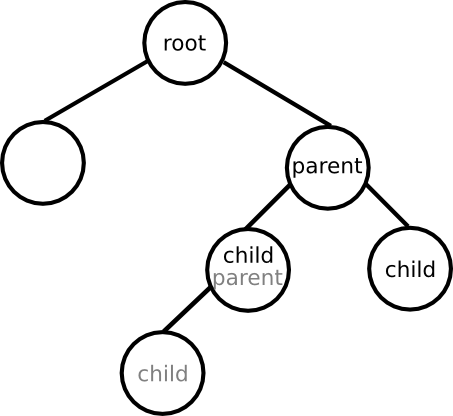
\includegraphics[width=0.8\textwidth]{figures/pcarent2.png}
\caption{Visar strukturen för parametrarna \textit{parent} och \textit{child} i Google drive.}
\label{fig:parentchild}
\end{figure}

\subsection{Lokal fillagring} \label{sec:local}
Den lokala filhanteringen infördes för att ge användaren ett alternativ utan extern kostnad och utan filutrymmesbegränsningar från externa tjänster. För att sköta uppladdningen, som är en central del av den lokala filhanteringen i och med att det inte går att importera filer likt från Google Drive eller Dropbox, implementerades en så kallad drag och släpp-uppladdning samt en formulärsuppladdning. Drag och släpp-uppladdningen innebär att användaren kan markera en eller flera filer på sin dator, dra dem till webbläsarfönstret där systemet är öppet och släppa dem. Systemet tar där vid och laddar upp filerna. När servern har tagit emot all uppladdningsdata från webbläsaren får filen ett slumpat filnamn och placeras i en mapp på servern.

\section{Gränssnitt}
För att utveckla gränssnittet användes främst HTML, CSS och Javascript. För att skriva CSS användes verktyget SASS\footnote{http://sass-lang.com/} (\textit{Syntactically Awesome Style Sheets}), vars syfte är att förenkla avancerade stilstrukturer genom att bland annat tillåta loopar, nästlade stilregler samt funktioner i CSS. Javascript användes för att göra gränssnittet snabbare för användaren genom att placera viss logik för utseendet i användarens webbläsare. Detta ledde till att webbläsarens DOM (\textit{Document Object Model}) kunde modifieras, och på så sätt snabbt ändra innehållet som presenteras. För detta användes Angularjs.

Sidans CSS kompletterades av ett par SASS- och CSS-ramverk för att underlätta utvecklandet. Bourbon\footnote{http://bourbon.io} användes för att tillhandahålla smidiga hjälpfunktioner, så kallade \textit{mixins} till SASS. För att kunna fylla tomma rutor i tjänsten användes kolumnsystemet Jeet\footnote{http://jeet.gs}. För att nollställa webbläsares olika standardinställningar, exempelvis länkars färger eller typsnitt, användes Normalize.css\footnote{http://necolas.github.io/normalize.css/}. Ikoner lades till för att göra knappar mer intuitiva vilket biblioteket Font Awesome\footnote{http://fontawesome.io}  användes för. För att visa att systemet laddar hem data, eller skicka data, användes Nprogress \footnote{http://ricostacruz.com/nprogress/}. Vidare användes knappar och textfält från Skeleton  \footnote{http://getskeleton.com}.

CSS-koden strukturerades upp i flera filer för att skapa en mer överskådlig struktur. Strukturen var uppdelad i följande kategorier: knappar, textfält, generell layout-struktur, huvudmeny, länkar, fillistor samt små individuella komponenter. 

\section{Testning}
Sedan version 1.9 utav Ruby har standardverktyget för testning varit Minitest \cite{rubychangelog}. Minitest erbjuder många delar som behövs för att kunna hantera testning. Det som användes mest var så kallade \textit{fixtures}, en exempelinstans utav en \textit{model} i systemet. Dessa användes för att säkerställa att systemet producerade de förändringar mot modellen som var väntade. Men även att de \textit{controllers} som fanns i systemet utförde rätt logik beroende på datan.

För att kontinuerligt säkerställa att projektet levde upp till de krav testerna specificerade användes tjänsten Travis CI, som testar att starta systemet och köra dess tester. Varje gång ny kod laddades upp gavs då ett resultat om hur testerna gick. Med denna kontinuerliga uppdatering gick det att via Github följa projektets status utan att ladda ned och starta det.

För testning av gränssnittet krävs dock ett program som kan simulera en webbläsares funktion genom att rendera Javascript, HTML och CSS. Då Travis CI redan hade ett sådant program som heter Phantomjs installerat valdes den. För att integrera Phantomjs med Minitest användes Capybara. Capybara är ett testningsverktyg och finns som tillägg till Minitest. Capybara erbjuder inte bara stöd för rendering utav javascript med Phantomjs utan ger också hjälpfunktioner för att göra tester som simulerar användarbeteende i gränsnittet, något som täcker in stora delar av både servern och gränsnittet.

De tester som utvecklarna lade mest tid på att implementera var tester för \textit{models}, \textit{controllers} samt integrationstester. Integrationstester är tester som testar ett användarbeteende och har väldigt enkla instruktioner, till exempel gå till startsidan och fyll inloggningsformuläret med dessa uppgifter och tryck sedan på logga in. Med dessa tester gavs en helhetsblick och en väldigt stor del av systemet testades med ett och samma test.

Tester skrevs efter att en funktion hade implementerats för att säkerställa att den önskade funktionaliteten skulle hålla i framtida utveckling av andra funktioner.

\section{Utvecklingsmetodik}
Genom att använda Scrum som utvecklingsmetodik gavs en bra grund och tydliga riktlinjer att följa under projektets gång.

\subsection{Roller}
Utvecklingsteamet bestod av fem personer där varje person fick en nyckelroll:

\subsubsection{Scrummästare}
Dennes ansvar innefattade att se till att teamet höll sig till de riktlinjer som fanns, sköta kommunikationen runt de mer administrativa bitarna (boka sal, bestämma arbetsdagar och så vidare) och hålla i scrummöten.

\subsubsection{Produktägare}
Produktägarens ansvar var att hålla kontakten med kund och se till att kundens krav omvandlades till scenarion och uppgifter. Det var även dennes ansvar att hålla ordning i produktbackloggen.

\subsubsection{Kodansvarig}
Dennes ansvar gick ut på att hitta ett bra system för att integrera nya delar i det befintliga systemet och sedan se till att detta system upprätthölls. 

\subsubsection{Testansvarig}
Dennes uppgift var att se till att systemet testades för att säkerställa att de krav som fanns uppnåddes och för att kontinuerligt jobba för att upptäcka brister i systemet.

\subsubsection{Dokumentansvarig}
Dokumentansvarig hade till uppgift att säkerställa att projektet blev ordentligt dokumenterat. Det var önskvärt att ha protokoll från kundmöten, gruppmöten med beslutsfattande karaktär och dokumentera skisser och liknande vid diskussioner kring systemets uppbyggnad.

\subsection{Händelser}
Hela utvecklingsperioden delades upp i mindre sprintar. Dessa sprintar hade en förutbestämd tid som inte kunde förlängas även om teamet upplevde att tiden inte räckte till. Varje sprint hade samma struktur. Vid uppstart hölls en sprintplanering där alla i teamet satte sig tillsammans för att gå igenom vilka scenarion från produktbackloggen som skulle ligga till grund i förestående tidsperiod. Det var viktigt att försöka hålla en god balans mellan tid och antalet valda scenarion. Teamet fick tillsammans utvärdera om de ansåg det möjligt att utföra alla scenarion innan sprintens avslut. När samtliga scenarier var valda bröts de ned i mindre delar och formades till specifika uppgifter. Det var önskvärt att hålla dessa uppgifter små och konkreta för att ha möjlighet att genomföra dessa under en arbetsdag. 

Inför varje arbetsdag i en sprint höll teamet ett dagligt scrummöte. Detta var ett kort möte på max 15 minuter där alla i teamet stod upp, utan datorer. Varje gruppmedlem fick under detta möte berätta vad de gjorde senast och vad de skulle göra under dagen. Detta gav alla en bra inblick i arbetet och en kort avstämning på hur teamet låg till tidsmässigt.

Den sista arbetsdagen i varje sprint ägnades åt de två avslutande sprintmötena. Det första av dessa var en sprintgranskning. Detta var ett tillfälle då hela teamet kunde diskutera det senaste projektinkrementet och hur arbetet hade fortskridit. Det första som gjordes på dessa möten var att gå igenom de scenarion som fanns inför sprinten och om dessa blivit avslutade. Eftersom målet med varje sprint var att ha en fungerande produkt med de krav som scenarierna representerade, gav denna genomgång en tydlig bild om hur effektivt gruppen arbetat. Nästa del i mötet var att diskutera de problem som uppstått under sprintens gång och hur dessa blivit lösta. Den sista delen av dessa möten ägnades åt att diskutera den dåvarande backloggen, vad som skulle göras härnäst och vilka faktorer som spelade roll inför nästa produktinkrement. 

Den sista aktiviteten i varje sprint var en sprintåterblick. Detta var ett möte där gruppen lade fokus på sina egna prestationer, de sociala relationerna i gruppen och de verktyg som använts. Detta var ett tillfälle där alla fick möjlighet att diskutera och påverka dessa aspekter för att jobba mot ett bättre arbetsklimat.

För att kunna skapa en realistisk bild över projektets storlek, vilka tidsramar projektet skulle delas upp i och hur mycket som skulle kunna åstadkommas under projektets gång skapades en tidsplan. För att ge en tydlig bild skapades ett Gantt-schema \cite{softwareeng} som ett kalkylark i teamets gemensamma Google Drive. Där samlades alla dagar i projektperioden. I schemat kunde deadlines, tänkta kundmöten, sprintarna och lediga perioder åskådliggöras på ett smidigt sätt. (BILAGA [])

För att få en överblick över vilken sprint som påbörjats och vilka uppgifter som skulle slutföras användes webbtänsten Trello, se figur \ref{fig:trello}, som scrumboard\cite{scrumboard}. Produktägaren skötte uppdateringen av pruduktbackloggen och sprintbackloggen i denna tjänst. Samtliga i gruppen hade fria händer att påbörja vilken uppgift som helst från sprintbackloggen. För att veta vem som påbörjat en uppgift märktes uppgiften med gruppmedlemmens namn. Övrig dokumentation som till exempel protokoll från sprintåterblick och sprintgranskning sköttes med hjälp av Google Drive. Även skisser på klassdiagram och programfunktionalitet sparades som bilder i Google Drive.

\begin{figure}[!H]
\centering
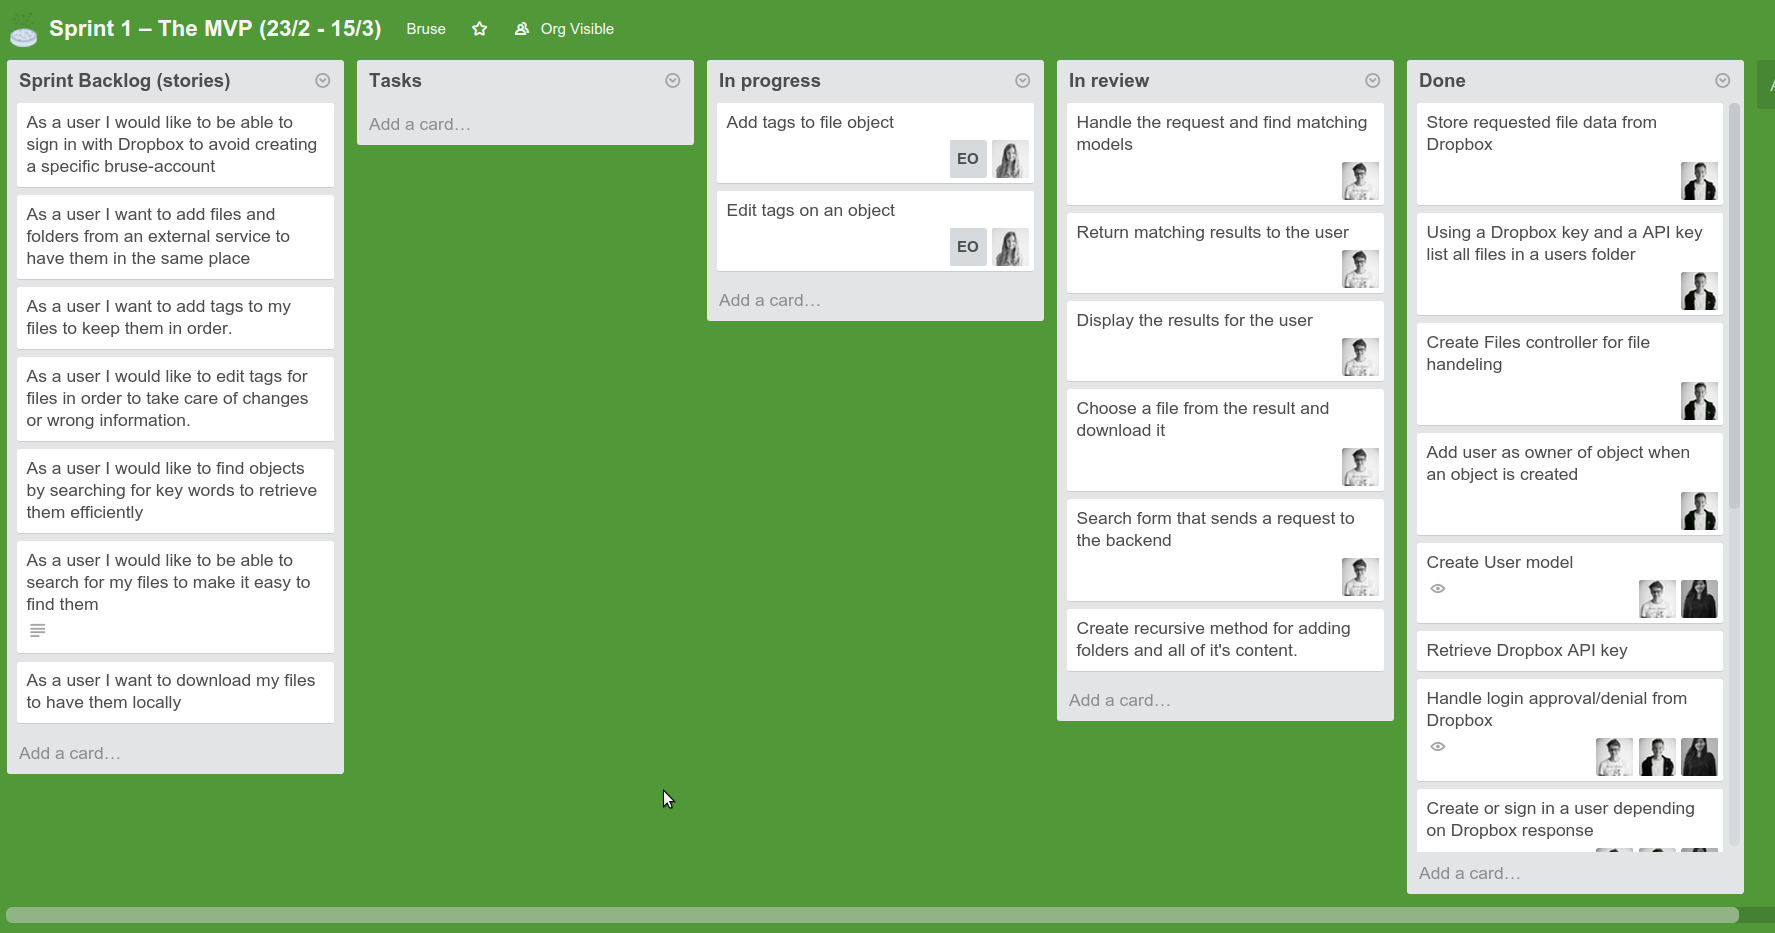
\includegraphics[width=0.8\textwidth]{figures/trello.png}
\caption{Scrumboard över sprint ett.}
\label{fig:trello}
\end{figure}

Här presenteras kort det fokus som fanns för varje sprint. Fullständiga sprintbackloggar går att se i (Bilaga []).

\subsubsection{Sprint 1 - MVP}
Målet med denna sprint var att ha en \textit{Minimum Viable Product}, MVP\cite{mvp} efter sprintavslutet. Något som var funktionellt och kunde visa på de problem som systemet skulle kunna lösa i ett senare skede. Fokus låg på att skapa en användare med Dropbox som fildatabas, importera filer från Dropbox till systemet och skapa nyckelord för filerna.

\subsubsection{Sprint 2 - Utveckla den tekniska funktionaliteten}
Fokus här var att göra filerna lättåtkomliga och sökbara. Dock uppkom det ett problem gällande Dropbox som fildatabas. En kostnad för ett SSL-certifikat (\textit{Secure Sockets Layer}), som används för att visa att en anslutning är krypterad, gjorde att teamet fick ändra riktning efter samråd med kund. Utöver sökningen blev det även fokus på att skapa ett mer modulärt system för att kunna lägga till flera typer av tjänster. Det teamet kom överens om var att implementera Google Drive och även skapa en lokal databas för egen server. 

\subsubsection{Sprint 3 - Tänka på användaren}
Under sprint tre hamnade fokus mer på systemets användare än den tekniska funktionaliteten. Ett flöde för systemets användande togs fram [BILD?], sökresultatens visning diskuterades [BILD?] samt utvecklades, och funktionalitet för drag och släpp-uppladdning påbörjades.

\subsubsection{Sprint 4 - Färdig produkt}
I den sista sprinten var det önskvärt att skapa ett användargränssnitt, få klart alla öppna scenarion och förbättra redan implementerad kod.

\section{Versionshantering och kodgranskning}
För versionshantering användes Git i kombination med Github genomgående i projektet. Git är ett distribuerat versionshanteringssystem där samtliga utvecklare har en komplett lokal kopia av hela projektet på dess egna datorer \cite{progit}.

För att underlätta vid konflikter och andra problem som uppstår då parallell utveckling av närliggande delar av projektet skedde användes Gits förgreningsfunktion. Förgreningar är en metod för att lösa problem som uppstår vid en linjär utveckling, där allt måste ske i en viss ordning. Flera utvecklare kunde jobba på olika komponenter utifrån en gemensam grund, och Git organiserade sedan hur dessa kunde sammanfogas på enklast möjliga vis \cite{progit}.

Inom förgreningen implementerades också en metod som populärt kallas \textit{feature branches}, som ungefär kan översättas till funktionalitetsgrenar \cite{gitflow}. Då en ny funktionalitet skulle implementeras i systemet skapade den ansvarige utvecklaren en förgrening. När utvecklaren var klar med det aktuella arbetet, skapades en förfrågan på Github (en \textit{pull request}) om att sammanfoga koden för den nya funktionaliteten med den befintliga. Innan koden sammanfogades fick den ansvarige utvecklaren återkoppling från resterande medlemmar i utvecklingsteamet om de blivande förändringarna och tilläggen. På så sätt skapades en trygghet för utvecklargruppen att det fanns en gemensam förståelse och konsensus kring det som skulle bli en del av den befintliga kodbasen.

\section{Refaktorering}
Refaktorering, det vill säga omstrukturering av kod, skedde med jämna mellanrum då till exempel en \textit{controller} blev för stor eller innehöll för många olika funktionaliteter. Den delades då upp för att tydliggöra vad de olika delarna hanterar. Exempelvis delades \textit{controllern} som hanterar användarnas filer upp i sex delar då den innehöll logik för olika delar av filhanteringen.
